% goodfellow
% 100 page
% Brownlee

% RNN

% backpropagation through time (BPTT) 

\section{Рекуррентные нейронные сети}

Что же делает рекуррентные сети такими особенными? Вопиющим 
ограничением классических нейронных сетей, рассмотренных ранее 
(а также сверточных нейронных сетей) 
является то, что их API слишком ограничен: 
они принимают на вход вектор фиксированного размера (например, изображение) 
и возвращают вектор фиксированного размера (например, вероятности 
различных классов). Более того, эти модели выполняют заданное отображение за 
фиксированное количество вычислительных шагов (например, количество слоев в модели). 
Основная причина, по которой рекуррентные нейронные сети настолько интересны 
заключается в том, что они позволяют нам работать с \textit{последовательностями} 
векторов: последовательность входных данных, выходных данных, или вообще и того, 
и другого. Рассмотрим несколько примеров:

\begin{figure}[h!]
    \centering
    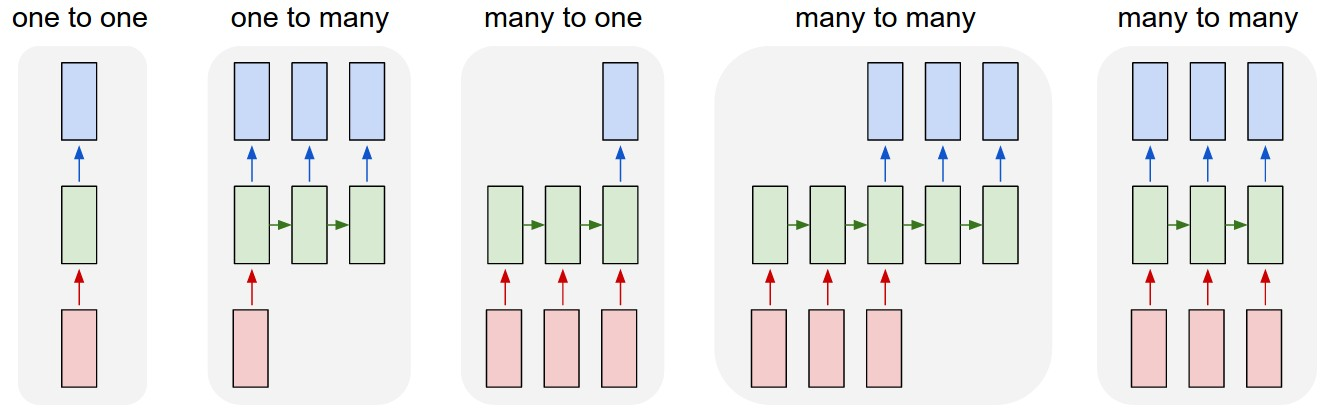
\includegraphics[width=1\textwidth, keepaspectratio]{rnn_sequences}
    \caption{Каждый прямоугольник представляет собой вектор, а стрелки - функции (например, 
    матричное умножение). Векторы входных данных представлены красным цветом, выходных - синим, 
    а зеленые содержат в себе состояние RNN (подробнее об этом далее). Слева направо: 
    (1) Классический метод обработки без RNN, на основании входа конечного размера производит 
    вывод конечного размера (например, классификация изображений). (2) Последовательность 
    в качестве выхода (например, описание изображений). (3) Последовательность в качестве входа 
    (например, анализ эмоциональной окраски, при котором заданное предложение 
    классифицируется как выражающее положительное или негативное настроение). (4) 
    Последовательность в качестве как входа, так и выхода (например, машинный перевод: 
    RNN считывает предложение на английском языке и возвращает его перевод на 
    французском языке). (5) Синхронизированная последовательность в качестве как входа, 
    так и выхода (например, классификация видео, где мы хотим назвать каждый кадр видео). 
    Заметим, что ни в одном из случаев на последовательности длин не наклыдывается 
    никаких предварительных ограничений, т.к. рекуррентное преобразование (зеленое) 
    фиксированно и может применяться сколько угодно раз.}
    \label{fig:rnn_sequences}
\end{figure}

Очевидно, что режим работы с последовательностями гораздо более мощный, по сравнению 
с фиксированными сетями, которые изначально обречены фиксированным количеством 
вычислительных шагов. По своей сути, RNN описывают программы. Вообще говоря, 
если проводить аналогию с универсальными теоремами аппроксимации, то известно, что 
RNN Тьюринг-полны в том смысле, что они могут симулировать поведение произвольных 
программ \cite{karpathy}.
\begin{center}
    \textit{Если обучение классических нейронных сетей можно назвать оптимизацией над 
    функциями, то обучение рекуррентных сетей можно назвать оптимизацией над программами.}
\end{center}

\noindent\textbf{Примечание} \hspace{10pt} Несмотря на то, что классические RNN сами по себе являются очень интересными, 
они обычно служат, своего рода, переходной ступенью к пониманию более 
продвинутых моделей, таких как LSTM и трансформеры (см. главы {\color{red} todo}):

\begin{figure}[h!]
    \centering
    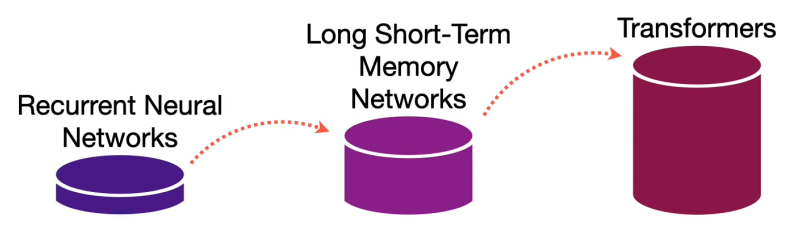
\includegraphics[width=0.8\textwidth, keepaspectratio]{RNN-steps}
    \caption{}
    \label{fig:RNN-steps}
\end{figure}

\newpage

\subsection{Архитектура рекуррентной нейронной сети}

Как же рекуррентным нейронным сетям удается работать с последовательностями 
произвольных размеров? У них это получается благодаря циклам, встроенным 
в них, позволяющим сохранять информацию.

\begin{figure}[h!]
    \centering
    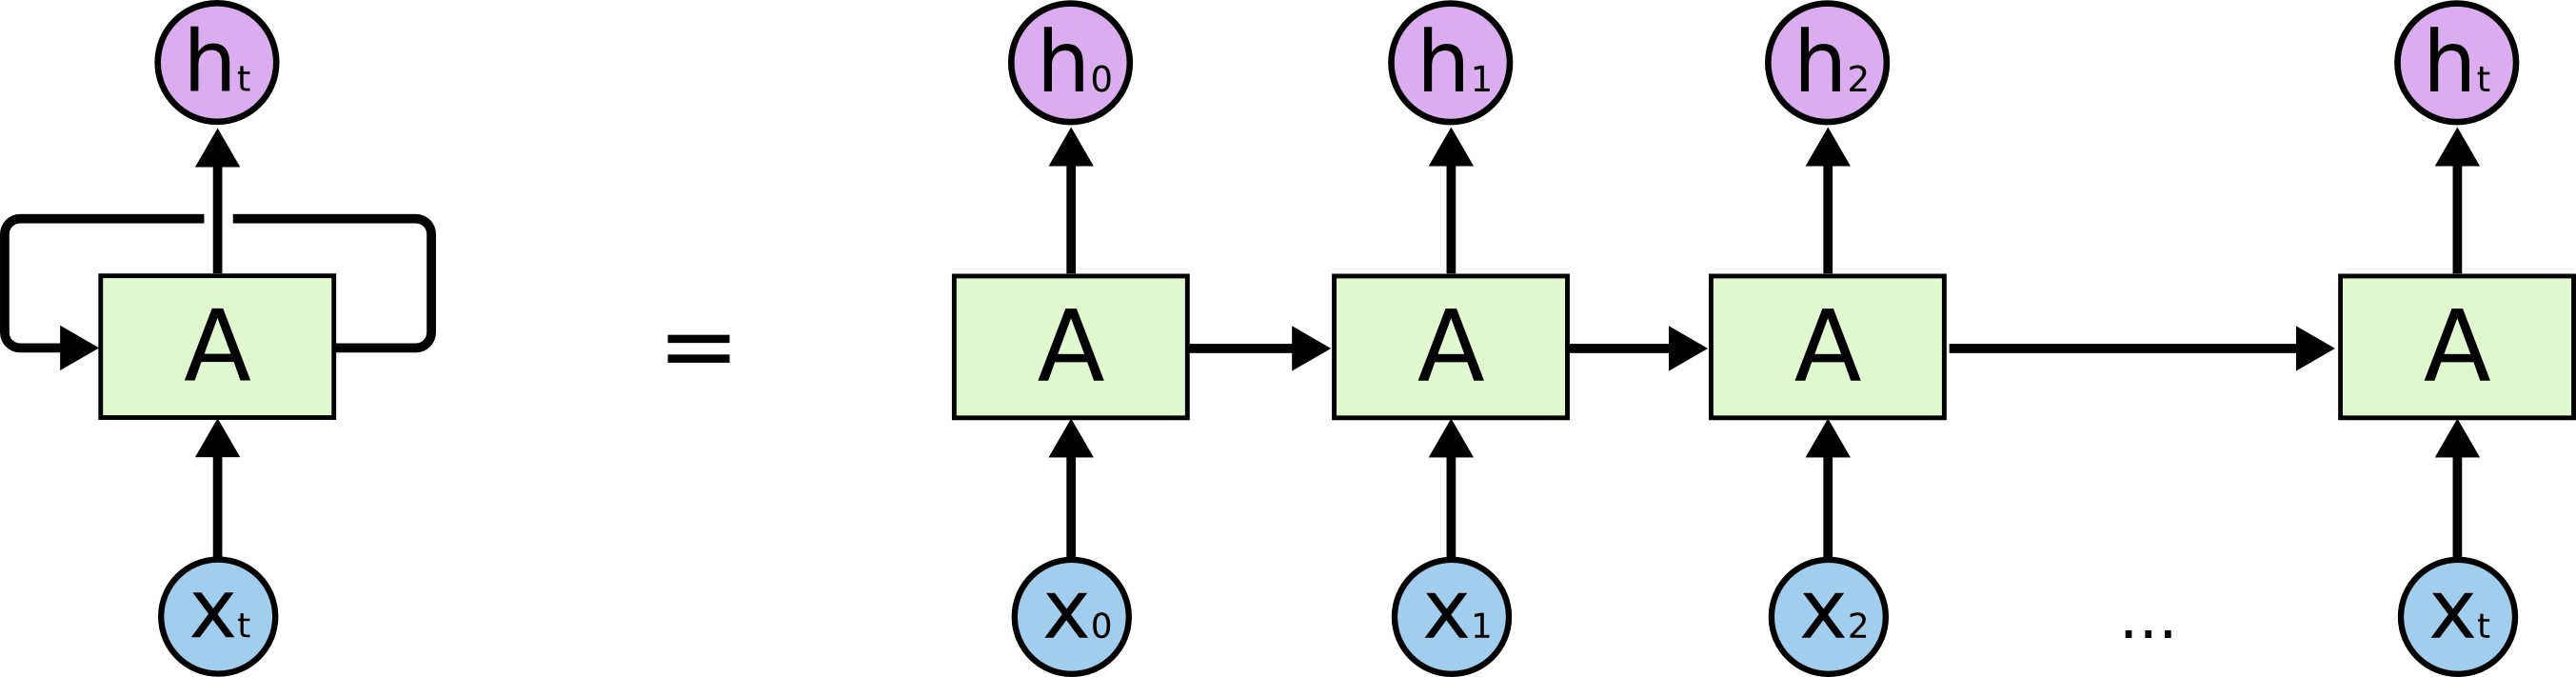
\includegraphics[width=0.8\textwidth, keepaspectratio]{RNN-unrolled}
    \caption{Схема рекуррентного слоя, где (слева)
    фрагмент нейронной сети $A$ принимает на вход некоторое значение $x_t$ 
    и возвращает некоторое значение $h_t$. Цикл позволяет информации 
    передаваться от одного шага сети к другому. Порой подобная 
    цикловая структура может сбить с толку, однак если его развернуть 
    (справа), то оказывается, что это очень похоже на классическую нейронную 
    сеть. О RNN можно думать как о множестве копий одной и той же сети, 
    каждая из которых передает сообщение своему последователю \cite{colah2}.}
    \label{fig:RNN-unrolled}
\end{figure}

Подобная цикловая структура позволяет обрабатывать последовательности 
данных произвольных размеров (стоит упомянуть, что в RNN мы используем 
одни и те же значения параметров (весов и смещений) 
внутри одного рекурентного слоя. Подобное разделение параметров позволяет 
применять и обобщать модель на примеры различной формы 
(в данном случае длины). Если бы у нас были различные параметры для 
каждого временного индекса, мы не смогли бы ни обобщить
модель на длины последовательностей, не встречавшиеся на этапе обучения, ни 
распространить статистическую силу на последовательности разной длины и 
на разные моменты времени).

\subsection{Прямой проход}

% add equations from Graves

% implement example

Разумеется на практике чаще используют RNN, состояющие не из одного 
рекуррентного слоя, а нескольких, чтобы получить, так называемые, 
\textbf{глубокие рекуррентые нейронные сети (depp RNNs)}. Такой подход 
позволяет нам, как и в случае многих слоев в FFNN и CNN, 
обучить иерархические зависимости между признаками, что на практие 
работает лучше однослойных сетей. 

\subsection{Обратный проход}

В силу своей природы, в RNN используется не классический метод обратного 
распространения ошибки (backpropagation) 
(см. главу {\color{red} todo}), а его модификация: 
\textbf{метод обратного распространения ошибки во времени 
(backpropagation through time (BPTT))} (разумеется существуют 
и другие алгоритмы, например RTRL, но в данной работе мы сфокусируемся на 
BPTT, тк он концепутально проще, популярнее и вычислительно эффективнее по времени 
(но не по памяти)). Принцип работы у BPTT такой же, как и у 
традиционного backprop. Единственное отличие заключается в том, что BPTT 
суммирует ошибки в каждый момент времени, когда, сети прямого распространения, 
в свою очердь, в этом не нуждаются, тк они не сохраняют значения параметров между 
слоями.

% why do people mostly use sigmoid activation functions 
% even though they cause so many problems and why not ReLU

% link to LSTM (from colah)
% Essential to these successes is the use of “LSTMs,” a very special kind of recurrent neural network which works, for many tasks, much much better than the standard version. Almost all exciting results based on recurrent neural networks are achieved with them. It’s these LSTMs that this essay will explore.

% LSTM

% (https://www.nickmccullum.com/python-deep-learning/vanishing-gradient-problem/#:~:text=The%20vanishing%20gradient%20problem%20has,success%20of%20recurrent%20neural%20networks)
% The most important solution to the vanishing gradient problem is a 
% specific type of neural network called Long Short-Term Memory Networks 
% (LSTMs), which were pioneered by Sepp Hochreiter and Jürgen Schmidhuber. 
% Recall that Mr. Hochreiter was the scientist who originally discovered 
% the vanishing gradient problem.

% LSTMs are used in problems primarily related to speech recognition, 
% with one of the most notable examples being Google using an LSTM for 
% speech recognition in 2015 and experiencing a 49\% 
% decrease in transcription errors.

% LSTMs are considered to be the go-to neural net for scientists 
% interested in implementing recurrent neural networks.

% GRU

% Transformer

% ensamble
